\documentclass[11pt,]{article}
\usepackage{lmodern}
\usepackage{amssymb,amsmath}
\usepackage{ifxetex,ifluatex}
\usepackage{fixltx2e} % provides \textsubscript
\ifnum 0\ifxetex 1\fi\ifluatex 1\fi=0 % if pdftex
  \usepackage[T1]{fontenc}
  \usepackage[utf8]{inputenc}
\else % if luatex or xelatex
  \ifxetex
    \usepackage{mathspec}
  \else
    \usepackage{fontspec}
  \fi
  \defaultfontfeatures{Ligatures=TeX,Scale=MatchLowercase}
\fi
% use upquote if available, for straight quotes in verbatim environments
\IfFileExists{upquote.sty}{\usepackage{upquote}}{}
% use microtype if available
\IfFileExists{microtype.sty}{%
\usepackage{microtype}
\UseMicrotypeSet[protrusion]{basicmath} % disable protrusion for tt fonts
}{}
\usepackage[margin=1in]{geometry}
\usepackage{hyperref}
\hypersetup{unicode=true,
            pdftitle={Probabilité et Statistique},
            pdfborder={0 0 0},
            breaklinks=true}
\urlstyle{same}  % don't use monospace font for urls
\usepackage{color}
\usepackage{fancyvrb}
\newcommand{\VerbBar}{|}
\newcommand{\VERB}{\Verb[commandchars=\\\{\}]}
\DefineVerbatimEnvironment{Highlighting}{Verbatim}{commandchars=\\\{\}}
% Add ',fontsize=\small' for more characters per line
\usepackage{framed}
\definecolor{shadecolor}{RGB}{248,248,248}
\newenvironment{Shaded}{\begin{snugshade}}{\end{snugshade}}
\newcommand{\KeywordTok}[1]{\textcolor[rgb]{0.13,0.29,0.53}{\textbf{#1}}}
\newcommand{\DataTypeTok}[1]{\textcolor[rgb]{0.13,0.29,0.53}{#1}}
\newcommand{\DecValTok}[1]{\textcolor[rgb]{0.00,0.00,0.81}{#1}}
\newcommand{\BaseNTok}[1]{\textcolor[rgb]{0.00,0.00,0.81}{#1}}
\newcommand{\FloatTok}[1]{\textcolor[rgb]{0.00,0.00,0.81}{#1}}
\newcommand{\ConstantTok}[1]{\textcolor[rgb]{0.00,0.00,0.00}{#1}}
\newcommand{\CharTok}[1]{\textcolor[rgb]{0.31,0.60,0.02}{#1}}
\newcommand{\SpecialCharTok}[1]{\textcolor[rgb]{0.00,0.00,0.00}{#1}}
\newcommand{\StringTok}[1]{\textcolor[rgb]{0.31,0.60,0.02}{#1}}
\newcommand{\VerbatimStringTok}[1]{\textcolor[rgb]{0.31,0.60,0.02}{#1}}
\newcommand{\SpecialStringTok}[1]{\textcolor[rgb]{0.31,0.60,0.02}{#1}}
\newcommand{\ImportTok}[1]{#1}
\newcommand{\CommentTok}[1]{\textcolor[rgb]{0.56,0.35,0.01}{\textit{#1}}}
\newcommand{\DocumentationTok}[1]{\textcolor[rgb]{0.56,0.35,0.01}{\textbf{\textit{#1}}}}
\newcommand{\AnnotationTok}[1]{\textcolor[rgb]{0.56,0.35,0.01}{\textbf{\textit{#1}}}}
\newcommand{\CommentVarTok}[1]{\textcolor[rgb]{0.56,0.35,0.01}{\textbf{\textit{#1}}}}
\newcommand{\OtherTok}[1]{\textcolor[rgb]{0.56,0.35,0.01}{#1}}
\newcommand{\FunctionTok}[1]{\textcolor[rgb]{0.00,0.00,0.00}{#1}}
\newcommand{\VariableTok}[1]{\textcolor[rgb]{0.00,0.00,0.00}{#1}}
\newcommand{\ControlFlowTok}[1]{\textcolor[rgb]{0.13,0.29,0.53}{\textbf{#1}}}
\newcommand{\OperatorTok}[1]{\textcolor[rgb]{0.81,0.36,0.00}{\textbf{#1}}}
\newcommand{\BuiltInTok}[1]{#1}
\newcommand{\ExtensionTok}[1]{#1}
\newcommand{\PreprocessorTok}[1]{\textcolor[rgb]{0.56,0.35,0.01}{\textit{#1}}}
\newcommand{\AttributeTok}[1]{\textcolor[rgb]{0.77,0.63,0.00}{#1}}
\newcommand{\RegionMarkerTok}[1]{#1}
\newcommand{\InformationTok}[1]{\textcolor[rgb]{0.56,0.35,0.01}{\textbf{\textit{#1}}}}
\newcommand{\WarningTok}[1]{\textcolor[rgb]{0.56,0.35,0.01}{\textbf{\textit{#1}}}}
\newcommand{\AlertTok}[1]{\textcolor[rgb]{0.94,0.16,0.16}{#1}}
\newcommand{\ErrorTok}[1]{\textcolor[rgb]{0.64,0.00,0.00}{\textbf{#1}}}
\newcommand{\NormalTok}[1]{#1}
\usepackage{longtable,booktabs}
\usepackage{graphicx,grffile}
\makeatletter
\def\maxwidth{\ifdim\Gin@nat@width>\linewidth\linewidth\else\Gin@nat@width\fi}
\def\maxheight{\ifdim\Gin@nat@height>\textheight\textheight\else\Gin@nat@height\fi}
\makeatother
% Scale images if necessary, so that they will not overflow the page
% margins by default, and it is still possible to overwrite the defaults
% using explicit options in \includegraphics[width, height, ...]{}
\setkeys{Gin}{width=\maxwidth,height=\maxheight,keepaspectratio}
\IfFileExists{parskip.sty}{%
\usepackage{parskip}
}{% else
\setlength{\parindent}{0pt}
\setlength{\parskip}{6pt plus 2pt minus 1pt}
}
\setlength{\emergencystretch}{3em}  % prevent overfull lines
\providecommand{\tightlist}{%
  \setlength{\itemsep}{0pt}\setlength{\parskip}{0pt}}
\setcounter{secnumdepth}{5}
% Redefines (sub)paragraphs to behave more like sections
\ifx\paragraph\undefined\else
\let\oldparagraph\paragraph
\renewcommand{\paragraph}[1]{\oldparagraph{#1}\mbox{}}
\fi
\ifx\subparagraph\undefined\else
\let\oldsubparagraph\subparagraph
\renewcommand{\subparagraph}[1]{\oldsubparagraph{#1}\mbox{}}
\fi

%%% Use protect on footnotes to avoid problems with footnotes in titles
\let\rmarkdownfootnote\footnote%
\def\footnote{\protect\rmarkdownfootnote}

%%% Change title format to be more compact
\usepackage{titling}

% Create subtitle command for use in maketitle
\newcommand{\subtitle}[1]{
  \posttitle{
    \begin{center}\large#1\end{center}
    }
}

\setlength{\droptitle}{-2em}
  \title{Probabilité et Statistique}
  \pretitle{\vspace{\droptitle}\centering\huge}
  \posttitle{\par}
  \author{}
  \preauthor{}\postauthor{}
  \date{}
  \predate{}\postdate{}

\usepackage{pst-plot,pst-node,pst-tree,pst-grad,pst-coil,pst-eps,pst-fill,multido}
\usepackage{array}
\usepackage{rotating}
\usepackage{amsmath}

\begin{document}
\maketitle

{
\setcounter{tocdepth}{6}
\tableofcontents
}
\newpage

\section{Introduction}\label{introduction}

L'homme à toujours utiliser un moyen d'échange à travers l'histoire.
Ceci allant de la Troc aux objects (précieux) d'échanges, jusqu'à
aujourd'hui l'utilisation la monnaie comme moyen d'échanges garantie (en
valeur) par les autorités publics. La quantité de la monnaie en
circulation, tel qu'elle soit, influe sur sa valeur (fiduciaire) à
l'instant \(t\). Le terme économique utilisé pour désigner la quantité
de monnaie en circulation est appelée \textbf{Masse Monétaire}. De fait
cette masse monétaire joue sur le prix des biens et services , et peut
être sources d'inflation (en cas d'augmentation de cette derniére),
c'est à dire une hausse des prix du fait de la baisse de sa valeur .
Mais elle peut aussi être source de désinflation voir déflation (en Cas
de baisse de cette derniére ) , c'est à dire une baisse de croissance
des prix voir une baisser des prix du fait de la hausse ainsi de sa
valeur.\\
Toutefois en europe du faits de l'intégration à l'Union Européenne, les
pays membres se voit des quotas de masse monétaire qui leurs sont
attribués, En fonction de la conjoncture économiques à la laquelle ils
font face. De ce fait, La quantité de monnaie fabriquée varie d'un pays
à l'autre. En outre de fait l'existence de la monnaie unique, le
processus d'intégration aujourd'hui va de paire avec le libre échange.
Ce qui rend le schéma plus complexe. En effet les pays membres, n'ayant
pas les mêmes quantités de monnaies fabriquées , peuvent se retrouver en
possession de monnaie originaires des autres pays voisins. Le defis
aujourd'hui étant de trouver un moyen de pouvoir connaitre la masse
monétaire en circulation qui est originaire du pays et la masse
monétaire en circulation qui non originaire du pays. Car la monnaie est
un levier en matiére de politique économique (plus précisement monétaire
et financiaire), et permet d'agir sur la conjoncture économique (c'est à
dire l'actualité économique du pays), avec son effet autant sur le long
terme que le court terme.\\
Le Principal probléme aujourd'hui face à ce genre de défis est surtout
dû au fait que les facteurs influants dans ce processus d'échanges ne
sont pas totalement maitrises ou sont souvent des facteurs latentes
(c'est à dire que l'on peut pas observer). En effet les facteurs comme
la compétivité d'un pays à un autre que ce soit structurelles ou prix,
ou les périodes de vacances\ldots{} Sont des facteurs que l'on connait
mais que l'on ne peut pas tout le temps maitriser.\\
Le deuxiéme principal probléme est ainsi lié au temps. En effet le temps
étant continue, l'échange de monnaie se font la plupart du temps avec un
décalage inter-temporels. Ce qui fait que la masse monétaire originaires
en circulation dans un pays, n'explique pas forcément la quantité
monnaie non originaires dans le même pays. Cela se comprend
particuliérement, dans la mesure ou la quanttié de base dans chaque pays
n'est jamais fixe même si les politiques au sain de l'Union Européenne
tendent à exiger des critéres de convergences comme celui-ci.

De ce fait nous essayerons à travers cette étude non pas d'expliquer ce
processus d'échanges, mais surtout d'essayer de voir dans un cadre trés
simple si l'on peu obtenir un équilibre statistique.\\
C'est à dire s'il existerait un temps \(t\) à partir duquel pour tout
échanges supplémentaires la masse monétaire originaire et la masse
étrangére serait plus ou moins stable dans un pays.

\newpage

\section{Modélisation}\label{modelisation}

\subsection{Processus avec N États}\label{processus-avec-n-etats}

Sous les hypothéses du processus d'échanges nous comprenons dés lors
qu'il faut essayer de voir comment ce systéme fonctionnerait avec
plusieurs États (comme c'est le cas en réalité).\\
Supposons d'abord :

\begin{itemize}
\item
  \emph{N} états dans un processus d'échanges , avec \emph{Q} la masse
  monétaire (totale) .
\item
  Le temp \emph{t} est discret et \emph{Q} est constant à travers le t
\item
  Un seul type de monnaie échangée (\(1\) euro) .
\end{itemize}

Donc à chaque temps \emph{t} nous avons:

\[Q=\sum_1^N q_{i}\]\\

\begin{flushright}
$q_{i}$ est la  de monnaie de L'état $i$ 
\end{flushright}

\begin{longtable}[]{@{}lllll@{}}
\toprule
\begin{minipage}[b]{0.08\columnwidth}\raggedright\strut
États\strut
\end{minipage} & \begin{minipage}[b]{0.11\columnwidth}\raggedright\strut
temps 1\strut
\end{minipage} & \begin{minipage}[b]{0.11\columnwidth}\raggedright\strut
temps 2\strut
\end{minipage} & \begin{minipage}[b]{0.10\columnwidth}\raggedright\strut
temps 3\strut
\end{minipage} & \begin{minipage}[b]{0.44\columnwidth}\raggedright\strut
\ldots{}\ldots{}\ldots{}.\strut
\end{minipage}\tabularnewline
\midrule
\endhead
\begin{minipage}[t]{0.08\columnwidth}\raggedright\strut
1\strut
\end{minipage} & \begin{minipage}[t]{0.11\columnwidth}\raggedright\strut
\(q_{1t_1}\)\strut
\end{minipage} & \begin{minipage}[t]{0.11\columnwidth}\raggedright\strut
\(q_{1t_2}\)\strut
\end{minipage} & \begin{minipage}[t]{0.10\columnwidth}\raggedright\strut
\(q_{1t_3}\)\strut
\end{minipage} & \begin{minipage}[t]{0.44\columnwidth}\raggedright\strut
\ldots{}\ldots{}\ldots{}\ldots{}.\strut
\end{minipage}\tabularnewline
\begin{minipage}[t]{0.08\columnwidth}\raggedright\strut
2\strut
\end{minipage} & \begin{minipage}[t]{0.11\columnwidth}\raggedright\strut
\(q_{2t_1}\)\strut
\end{minipage} & \begin{minipage}[t]{0.11\columnwidth}\raggedright\strut
\(q_{2t_2}\)\strut
\end{minipage} & \begin{minipage}[t]{0.10\columnwidth}\raggedright\strut
\(q_{2t_3}\)\strut
\end{minipage} & \begin{minipage}[t]{0.44\columnwidth}\raggedright\strut
\ldots{}\ldots{}\ldots{}..\strut
\end{minipage}\tabularnewline
\begin{minipage}[t]{0.08\columnwidth}\raggedright\strut
.\strut
\end{minipage} & \begin{minipage}[t]{0.11\columnwidth}\raggedright\strut
.\strut
\end{minipage} & \begin{minipage}[t]{0.11\columnwidth}\raggedright\strut
.\strut
\end{minipage} & \begin{minipage}[t]{0.10\columnwidth}\raggedright\strut
.\strut
\end{minipage} & \begin{minipage}[t]{0.44\columnwidth}\raggedright\strut
\ldots{}\ldots{}\ldots{}\ldots{}.\strut
\end{minipage}\tabularnewline
\begin{minipage}[t]{0.08\columnwidth}\raggedright\strut
.\strut
\end{minipage} & \begin{minipage}[t]{0.11\columnwidth}\raggedright\strut
.\strut
\end{minipage} & \begin{minipage}[t]{0.11\columnwidth}\raggedright\strut
.\strut
\end{minipage} & \begin{minipage}[t]{0.10\columnwidth}\raggedright\strut
.\strut
\end{minipage} & \begin{minipage}[t]{0.44\columnwidth}\raggedright\strut
\ldots{}\ldots{}\ldots{}\ldots{}..\strut
\end{minipage}\tabularnewline
\begin{minipage}[t]{0.08\columnwidth}\raggedright\strut
.\strut
\end{minipage} & \begin{minipage}[t]{0.11\columnwidth}\raggedright\strut
.\strut
\end{minipage} & \begin{minipage}[t]{0.11\columnwidth}\raggedright\strut
.\strut
\end{minipage} & \begin{minipage}[t]{0.10\columnwidth}\raggedright\strut
.\strut
\end{minipage} & \begin{minipage}[t]{0.44\columnwidth}\raggedright\strut
\ldots{}\ldots{}\ldots{}\ldots{}\strut
\end{minipage}\tabularnewline
\begin{minipage}[t]{0.08\columnwidth}\raggedright\strut
.\strut
\end{minipage} & \begin{minipage}[t]{0.11\columnwidth}\raggedright\strut
.\strut
\end{minipage} & \begin{minipage}[t]{0.11\columnwidth}\raggedright\strut
.\strut
\end{minipage} & \begin{minipage}[t]{0.10\columnwidth}\raggedright\strut
.\strut
\end{minipage} & \begin{minipage}[t]{0.44\columnwidth}\raggedright\strut
\ldots{}\ldots{}\ldots{}\ldots{}.\strut
\end{minipage}\tabularnewline
\begin{minipage}[t]{0.08\columnwidth}\raggedright\strut
N\strut
\end{minipage} & \begin{minipage}[t]{0.11\columnwidth}\raggedright\strut
\(q_{Nt_1}\)\strut
\end{minipage} & \begin{minipage}[t]{0.11\columnwidth}\raggedright\strut
\(q_{Nt_2}\)\strut
\end{minipage} & \begin{minipage}[t]{0.10\columnwidth}\raggedright\strut
\(q_{Nt_3}\)\strut
\end{minipage} & \begin{minipage}[t]{0.44\columnwidth}\raggedright\strut
\ldots{}\ldots{}\ldots{}\ldots{}\ldots{}\strut
\end{minipage}\tabularnewline
\begin{minipage}[t]{0.08\columnwidth}\raggedright\strut
------\strut
\end{minipage} & \begin{minipage}[t]{0.11\columnwidth}\raggedright\strut
--------\strut
\end{minipage} & \begin{minipage}[t]{0.11\columnwidth}\raggedright\strut
--------\strut
\end{minipage} & \begin{minipage}[t]{0.10\columnwidth}\raggedright\strut
----------------\strut
\end{minipage} & \begin{minipage}[t]{0.44\columnwidth}\raggedright\strut
---------------------------\strut
\end{minipage}\tabularnewline
\begin{minipage}[t]{0.08\columnwidth}\raggedright\strut
Masse monétaire\strut
\end{minipage} & \begin{minipage}[t]{0.11\columnwidth}\raggedright\strut
Q=\(\sum_1^Nq_{it_1}\)\strut
\end{minipage} & \begin{minipage}[t]{0.11\columnwidth}\raggedright\strut
Q=\(\sum_1^Nq_{it_2}\)\strut
\end{minipage} & \begin{minipage}[t]{0.10\columnwidth}\raggedright\strut
Q=\(\sum_1^Nq_{it_3}\)\strut
\end{minipage} & \begin{minipage}[t]{0.44\columnwidth}\raggedright\strut
\ldots{}\ldots{}\ldots{}\ldots{}.\strut
\end{minipage}\tabularnewline
\bottomrule
\end{longtable}

la visualisation de ce genre de processus est complexe compte tenue des
interactions qu'ils peuvent y avoir entre les états.

\subsection{Processus à Deux États}\label{processus-a-deux-etats}

\subsubsection{Chaine de Markov}\label{chaine-de-markov}

Nous allons maintenant considérer un systéme d'échange à deux états.
Nous conservons entre autre les hypothéses précédentes.

Soit :

\begin{itemize}
\item
  \textbf{A} et \textbf{B} deux états.
\item
  Nous supposons le temps discret, \(N_A\) et \(N_B\) la quantité de
  monnaie respective à ces deux pays, avec \(N_A \leq N_B\).
\item
  À chaque temps (\(t \in \mathbb{N}\)), nous avons ce phénoméne qui se
  produit :
\end{itemize}

\[code 1\]

\begin{itemize}
\tightlist
\item
  Soit \(X(t)\) la variable aléatoire associée à l'évenement ``la
  quantité de piéce de un euro dans A à l'instant t'',
  \(\forall t\in \mathbb{N}\), \(X(t)\in\) {[}0,\(N_A\){]}.
\end{itemize}

\[code2\]

Soit \(k \in [1,N_A-1]\), soit \(t \in \mathbb{N}\), À l'état \(k\)
(c'est à dire \(X(t)=k\)) :

\begin{itemize}
\tightlist
\item
  Si \(X(t+1)=k-1\) , alors il y aura \(k-1\) piéces de \emph{1} euro de
  \(A\) dans le pays \(A\) . et il y aura \(N_A-(k-1)\) piéces de
  \emph{1} euro de \(B\) dans \(A\), car la piéce ayant quittée \(A\)
  était de \(A\) (avec probabibité \(\frac{k}{N_A}\)) et celle qui est
  arrivée dans \(A\) était originaire de \(B\) (avec probabilité
  \(\frac{N_B-(N_A-k)}{N_B}\) ).\\
  En sachant que les deux événements sont indépendants, donc la
  probabilité de transition est la suivante:
\end{itemize}

\begin{equation} 
\begin{split}
\mathbb{P}(X(t+1) =k-1|X(t)=k) &=\frac{k}{N_A}(\frac{N_B-(N_A-k)}{N_B} ) \\
&=\frac{k}{N_A}(1-\frac{N_A}{N_B}+\frac{k}{N_B})\\
&=\frac{k}{N_A}(1-\rho+\rho \frac{k}{N_A})  \\
\end{split}
\end{equation}

\begin{flushright}
*\emph{Avec $\rho=\frac{N_A}{N_B}$}
\end{flushright}

\begin{itemize}
\tightlist
\item
  Si \(X(t+1)=k+1\), alors il y aura \(k+1\) piéces de \emph{1} euro de
  \(A\) dans \(A\) et \(N_A-(k+1)\) piéces de \emph{1} euro de \(B\)
  dans \(A\) , car la piéce ayant quittée \(A\) était de \(B\) (avec
  probabilité \(\frac{N_A-k}{N_A}\)) et celle qui est arrivée dans \(A\)
  était originaire de \(A\) (avec probabilité \(\frac{N_A-k}{N_B}\)).
\end{itemize}

En sachant que dans cas aussi les deux événements sont indépendants,
donc la probabilité de transition est la suivante:\\

\begin{equation} 
\begin{split}
\mathbb{P}(X(t+1) =k+1|X(t)=k) &=(\frac{N_A-k}{N_A})(\frac{N_A-k}{N_B})\\
&=(1-\frac{k}{N_A})(\frac{N_A}{N_B}-\frac{k}{N_B})\\
&=(1-\frac{k}{N_A})(\rho-\rho\frac{k}{N_A})\\
&=\rho(1-\frac{k}{N_A})^2
\end{split}
\end{equation}

Si \(X(t+1)=k\), alors il y aura \(k\) piéces de \emph{1} euro de \(A\)
dans \(A\) et \(N_A-k\) piéces de \(B\) dans \(A\). Dans ce cas il y a
deux possibilité:

\begin{itemize}
\item
  la piéce ayant quittée \(A\) était de \(A\) (avec probabilité
  \(\frac{k}{N_A}\))et celle arrivée dans dans \(A\) était originaire de
  \(A\) (avec probabilité \(\frac{N_A-k}{N_B}\)).
\item
  Ou bien la piéce ayant quitté \(A\) était de \(B\) (avec probabilité
  \(\frac{N_A-k}{N_A}\)) et celle qui est arrivée dans \(A\) était
  originaire de \(B\) (avec probabilité \(\frac{N_B-(N_A-k)}{N_B}\)).
\end{itemize}

Et sachant que les événements sont deux à deux disjoints, la probabilité
de transition est la suivante:

\begin{equation} 
\begin{split}
\mathbb{P}(X(t+1) =k|X(t)=k)  
&=(\frac{k}{N_A})(\frac{N_A-k}{N_B})+(\frac{N_A-k}{N_A})(\frac{N_B-(N_A-k)}{N_B})\\
&=\frac{k}{N_A}\rho(1-\frac{k}{N_A})+(1-\frac{k}{N_A})(1+\rho+\rho\frac{k}{N_A})\\
&=(1-\frac{k}{N_A})(1+\rho+2\rho\frac{k}{N_A})\\
\end{split}
\end{equation}

\begin{itemize}
\item
  Pour \(X(t)=0\), \(\mathbb{P}(X(t+1)=1|X(t)=0)=1\). Et pour
  \(X(t)=N_A\),\\
  \(\mathbb{P}(X(t+1)=N_A-1|X(t)=N_A)=1\)
\item
  Soit \(j,i \in [0,N_A]\) tel que \(|i-j|\geq 2\),
  \(\mathbb{P}(X(t+1)=j|X(t)=i)=\mathbb{P}(X(t+1)=i|X(t)=j)=0\).
\end{itemize}

Nous pouvons ainsi dire que la probabilité dans un état (de 0 à \(N_A\))
ne dépend que de l'état précedent dans notre modéle. Donc nous pouvons
bien affirmer que l'on a une chaine de markov homogéne finie avec la
matrice de transition suivante.

\[
\left(\begin{array}{cccccccccccccc}
\\r_0&p_0&&&&&&&&&&&&\\  
q_2&r_2&p_2&&&&&&&&&&&\\  
&q_3&r_3&p_3&&&&&&&&&&\\  
&&.&.&.&&&&&&&&&\\  
&&&.&.&.&&&&&&(0)&&\\  
&&&&.&.&.&&&&&&&\\  
&&&&&.&.&.&&&&&&\\  
&&&&&&q_k&r_k&p_k&&&&&\\  
&&&&&&&.&.&.&&&&\\  
&&&&&&&&.&.&.&&&\\  
&&&(0)&&&&&&.&.&.&&\\  
&&&&&&&&&&q_{N_A-1}&r_{N_A-1}&p_{N_A-1}&\\  
&&&&&&&&&&&q_{N_A}&r_{N_A}&p_{N_A}\\
\end{array}\right)\]

Avec \(\forall t \in \mathbb{N},\forall k \in [1,N_A-1]\):

\[ \Rightarrow \left\{
  \begin{array}{rcr}
  r_k=&\mathbb{P}(X(t+1)=k|X(t)=k)=&(1-\frac{k}{N_A})(1-\rho+2\rho\frac{k}{N_A})\\
  p_k=&\mathbb{P}(X(t+1)=k+1|X(t)=k)=&\rho(1-\frac{k}{N_A})^2\\
  q_k=&\mathbb{P}(X(t+1)=k-1|X(t)=k)=&\frac{k}{N_A}(1-\rho+\rho \frac{k}{N_A}) \\
\end{array}
\right.
\]

\(r_0=r_N=0,q_{N_A-1}=p_0=1\)

Dans le cas ou \(N_A=N_B=N\), entrainant \(\rho=1\) ,nous avons :

\[ \Rightarrow \left\{
  \begin{array}{rcr}
  r_k=&\mathbb{P}(X(t+1)=k|X(t)=k)=&\frac{2k}{N_A}(1-\frac{k}{N_A})\\
  p_k=&\mathbb{P}(X(t+1)=k+1|X(t)=k)=&(1-\frac{k}{N_A})^2\\
  q_k=& \mathbb{P}(X(t+1)=k-1|X(t)=k)=& (\frac{k}{N_A})^2\\
\end{array}
\right.
\]

\subsubsection{Propriété de la chaine}\label{propriete-de-la-chaine}

• \textbf{Périodicité}\\
Soit \(x \in E\) et \(R(x)=\{t \in N^*, P^t(x,x)>0 \}\) , On appele
période de \(x\) le PGCD(R(X)) ,si la période est égale 1 alors la
chaine est Apériodique.\\
Donc la chaine etudié est Aperiodique.

• \textbf{irréductible}\\
Car pour tout \(x, y\in[0,N_A]\) avec \(|x-y|\leq 1\) nous avons
\(x R y\) et \(yRx\)

\subsubsection{Mesure invariante}\label{mesure-invariante}

Sachant que la chaine est homogéne finie irreductible et Apériodique un
théoréme affirme qu'elle admet\\
une mesure invariante \(\pi\) ,tel que \(\pi=\pi P\), et pour toute
mesure initiale \(\mu\) et tout \(k \in [0,N_A]\) , T assez grand :\\
\[\frac{1}{T}\sum_{t=0}^{T-1}\mathbb{1}_{\{X(t)=k\}} \Longrightarrow \pi(k) \hspace{20mm} (ps) \]

\[ \pi=\pi P \Rightarrow \left\{
  \begin{array}{rcr}
    \pi_0=&r_0\pi_0+q_1\pi_1 \\
   \pi_1=&p_0\pi_0+r_1\pi_1+q_2\pi_2 \\
   .\\
   .\\
   \pi_k=&p_{k-1}\pi_{k-1}+r_k+q_{k+1}\\
   .\\
   .\\
   \pi_{N_A}=&p_{N_A-1}\pi_{N_A-1}+r_{N_A}+q_{N_A+1}
  \end{array}
\right.
  \]

\begin{flushright}
  $r_k+p_k+q_k=1$
  \end{flushright}

\[
  \Rightarrow \left\{
  \begin{array}{rcr}
  (1-r_0)\pi_0=&q_1\pi_1\\
  (1-q_1-r_1)\pi_1=&q_2\pi_2\\
  ...&\\
  ...&\\
  (1-q_k-r_k)\pi_k=&q_{k+1}\pi_{k+1}\\
    ...&\\
  ...&\\
  (1-q_{N_A-1}-r_{N_A-1})\pi_{N_A-1}=&q_{N_A}\pi_{N_A}
  \end{array}
  \right.
  \Rightarrow \left\{ \begin{array}{rcr}
  p_0\pi_0=&q_1\pi_1\\
  p_1\pi_1=&q_2\pi_2\\
  ...&\\
  ...&\\
  p_k\pi_k=&q_{k+1}\pi_{k+1}\\
    ...&\\
  ...&\\
  p_{N_A-1}\pi_{N_A-1}=&q_{N_A}\pi_{N_A}
  \end{array}
  \right.
  \]

En écrivant en fonction \(\pi_0\) \[ 
\Rightarrow \left\{ \begin{array}{rcr}
  \pi_1=&\frac{p_0}{q_0}\pi_0\\
  \pi_2=&\frac{p_0p_1}{q1q_2}\pi_0\\
  ...&\\
  ...&\\
  p_k\pi_k=&\frac{p_{k-1}....p_0}{q_{k}....q_1}\pi_0\\
    ...&\\
  ..&\\
  p_{N_A}\pi_{N_A}=&\frac{p_{N_A-1}...p_0}{q_{N_A}...q_1}\pi_{0}
  \end{array}
  \right. 
  \]\\

\begin{center}
 Avec ,$ \sum_{k=0}^{N_A} \pi_k=1$
  \end{center}

\begin{itemize}
\tightlist
\item
  Dans le cas ou \(N_A=N_B=N\) nous avons :
\end{itemize}

\[\pi_k=\frac{p_{k-1}....p_0}{q_{k}....q_1}\pi_0=\frac{\prod_0^k(\frac{N-k'+1}{N})^2}{\prod_1^k(\frac{k'}{N})^2}\pi0=\frac{\prod_0^k(N-k'+1)^2}{\prod_1^k k'^2}=\frac{(N!)^2}{k!^2(N-k)^2}\pi_0=\binom{N}{k}^2\pi_0
\]\\
or \(\sum_0^N\pi_k=1\) \(\Rightarrow\)
\(\sum_0^N\binom{N}{k}^2\pi_0=\pi_0 \binom{2N}{N}=1\) \(\Rightarrow\)
\(\pi_0=\binom{2N}{N}^{-1}\)

Donc :

\begin{itemize}
\tightlist
\item
  \[\pi_k=\binom{N}{k}^2\pi_0=\frac{\binom{N}{k}^2}{\binom{2N}{N}}=\frac{\binom{N}{k}\binom{N}{N-k}}{\binom{2N}{N}}\]
\end{itemize}

D'ailleurs cela correspond à une loi hypergéométrique de raison N, un
équilibre avec une répartition des piéces de \(1\) euros aléatoire entre
les deux états.

En translatant le probléme pour le cas \(N_A \leq N_B\):\\
\[\Rightarrow \pi_k =\frac{p_{k-1}....p_0}{q_{k}....q_1}\pi_0=\frac{\rho^k\frac{1}{N_A^k}(N_A(N_A-1)...(N_A-(k-1)) )^2}{\frac{k!}{N_A^k}(1-\frac{N_A}{N_B}+\frac{k}{N_B}))....(1-\frac{N_A}{N_B}+\frac{1}{N_B})) }\pi_0\\=\frac{\rho^k \frac{N_A!^2}{(N_A-k)!^2} }{\frac{k!}{N_B^k}((N_B-(N_A-k))...(N_B-(N_A-1))}\pi_0 =\]

\[= \frac{\rho^k \frac{N_A!^2}{(N_A-k)!^2 }}{ \frac{k!}{N_B^k} \frac{N_B!}{(N_B-N_A)!} }\pi_0=
  \frac{N_A!^2}{(N_A-k)!^2} * \frac{1}{N_A^k k!}\frac{(N_B-N_A)!}{N_B!}\\
   \approx \frac{\binom{N_A}{k}\binom{N_B}{N_A-k}}{\binom{N_A+N_B}{N_A}}\]

Nous comprenons dés lors que ce modéle est trés simpliste comparé à la
réalité. Mais l'intérêt est surtout de voir au bout de combien de temps
nous nous s'approcherons de l'équilibre.

Le graphique ci-dessous correspond à une simulation avec
\(N_A=20, N_B=20\) et \(X(0)=20\), c'est à dire que l'état \(A\)
possédait au départ 20 piéces de \(1\) euro qu'elle a fabriqué et 0
piéce de l'état \(B\).

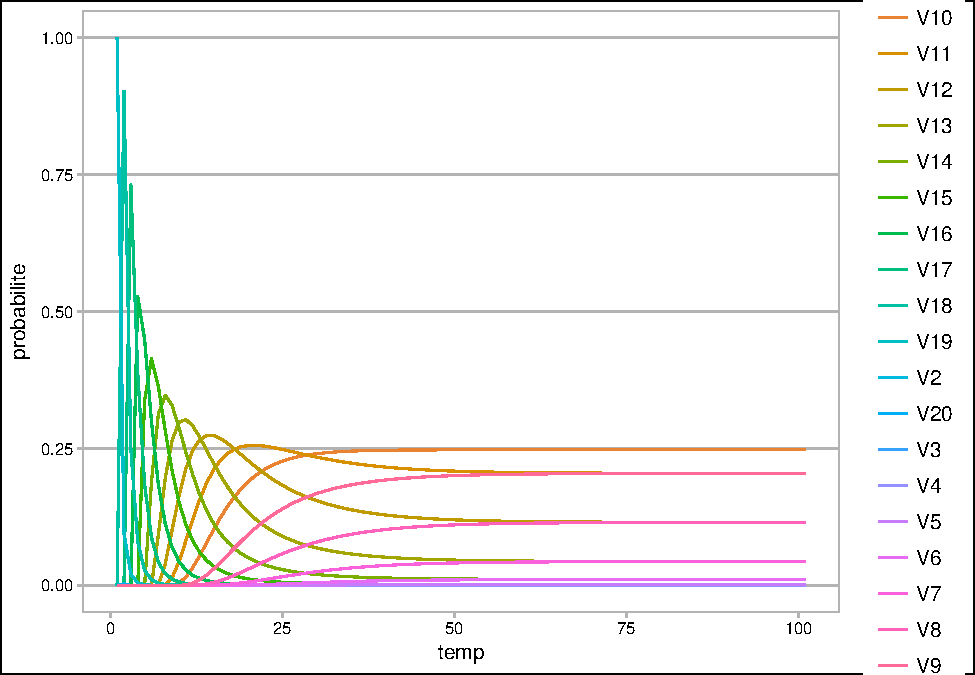
\includegraphics{money_exchange_files/figure-latex/unnamed-chunk-3-1.pdf}

\begin{itemize}
\tightlist
\item
  Nous pouvons constaté que à partir du temp \(t=60\) un équilibre
  commence à se créer, avec \(X(t)\) plus problable d'être entre
  \([8,11]\). Ce qui représente la moitié plus ou moins.
\end{itemize}

Le graphique ci-dessous le cas ou \(\rho=\frac{1}{2}\), c'est à dire
\(N_A=10,N_B=20\) et l'état \(A\) possédait au départ 10 piéces de \(1\)
euro qu'elle a fabriqué et 0 piéce de l'état \(B\).

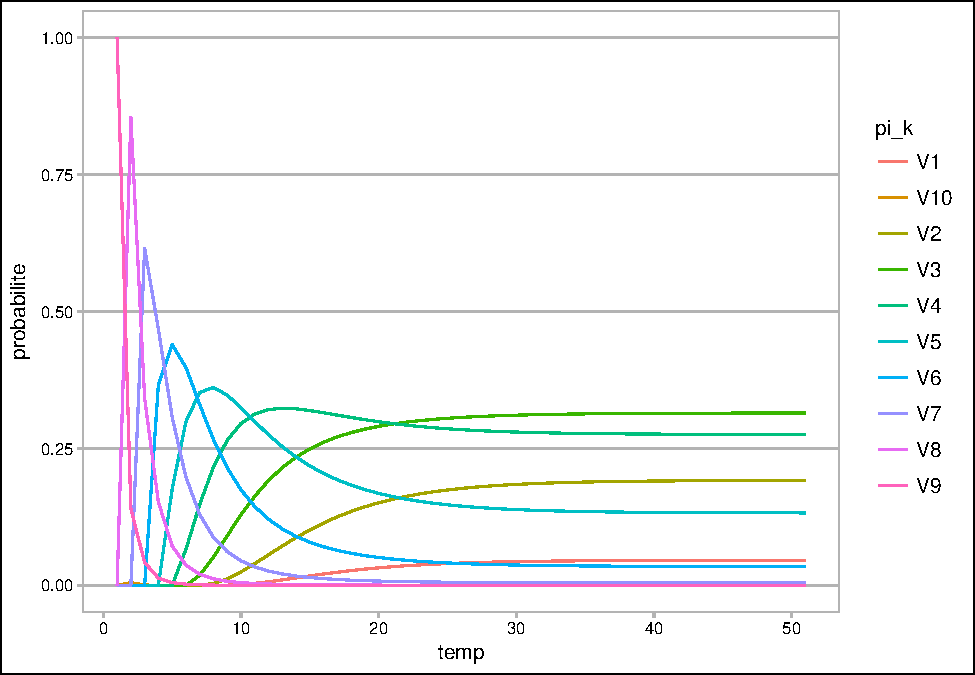
\includegraphics{money_exchange_files/figure-latex/unnamed-chunk-4-1.pdf}

\begin{itemize}
\tightlist
\item
  Nous pouvons remarquer avec ce graphique, comparé au cas précedent,
  que le temps pour atteindre l'équilibre stationnaire est deux fois
  plus petit. avec \(X(t)\) plus problable d'être entre \([2,5]\). Ce
  qui représente la moitié plus ou moins.
\end{itemize}

• Le graphique ci-dessous represente le cas ou \(\rho\approx 0.125\), ce
qui est proche de zéro. C'est à dire \(N_A=10,N_B=800\) et l'état \(A\)
possédait au départ 10 piéces de \(1\) euro qu'elle a fabriquée et 0
piéce de l'état \(B\).

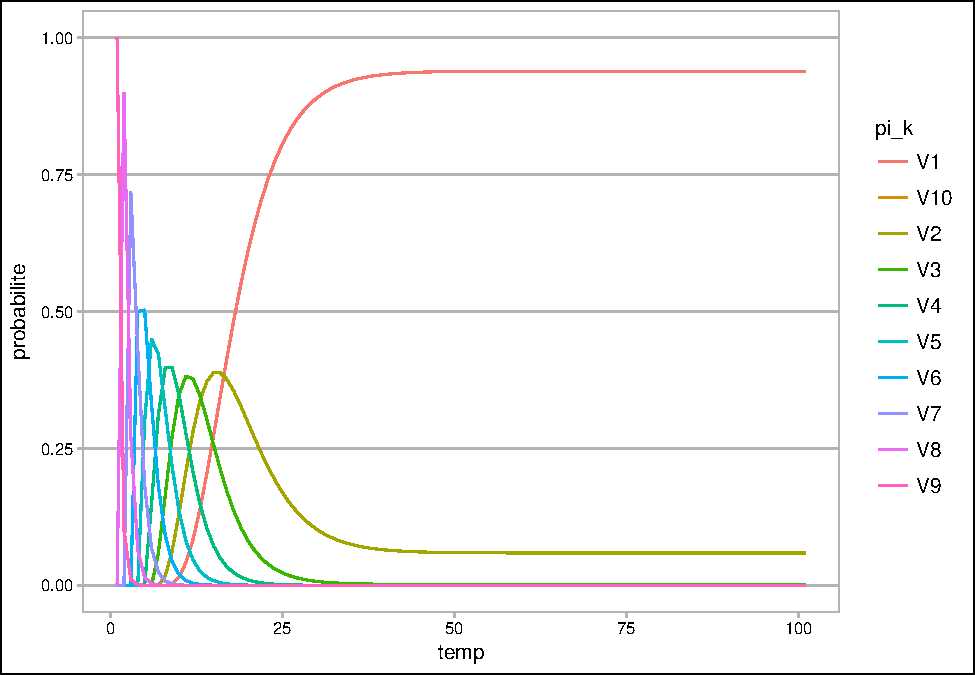
\includegraphics{money_exchange_files/figure-latex/unnamed-chunk-5-1.pdf}

\begin{itemize}
\tightlist
\item
  En dépit du fait que la convergence se fait beaucoup plus tôt que
  précédemment, nous sommes presque sur de la convergence \(X(t)=2\)
  (avec \(\approx\) 75\% de chance) c'est qui represente environ 10\%
  des piéces fabriquées par \(A\)
\end{itemize}

Pour conclure cette partie nous pouvons dire que la valeur de \(\rho\)
joue sur la vitesse de convergence vers l'équilibre. En effet une valeur
de \(\rho\) trop proche de zéro entraine une vers convergence beaucoup
plus rapide dans le temps contrairement à valeur de \(\rho\) proche de 1
( \(N_A\) pas trop différent de \(N_B\)) .

\subsubsection{Cas particulier}\label{cas-particulier}

Dans cette partie nous allons un deuxiéme modéle possible. Nous
considérons \(N_A=N\) et les piéces fabriquées par l'états sont reconnus
par leurs numéros de fabrications.\\
L'idée étant que à chaque instant \(t\) une piéce parmi celles
fabriquées par l'état \(A\) est prie de maniére uniforme et change
automatiquement de pays. la différence par rapport au modéle d'avant se
base sur le fait que un seul pays ici est fabriquant des piéces. le but
ici sera aussi voir au bout de combien de temps pourrions atteindre un
équilibre. Ce modéle prend en compte le fait que en réalité les échanges
ne se font pas forcément de maniére simultanée.

\begin{itemize}
\tightlist
\item
  Soit l'état \(X(t)=k\) ,avec \(k \in\) {[}1,N-1{]}:
\end{itemize}

Si \(X(t+1)=k-1\) alors la piéce tirée était dans A (avec probabilité
\(\frac{k}{N}\)).\\
Si \(X(t+1)=k+1\) alors la piéce tirée était dans B (avec probabilité
\(\frac{N-k}{K}\)). Si \(k=0\) alors forcément \(X(t+1)=1\) ou \(k=N\)
alors forcément \(X(t+1)=N-1\).\\
De ce fait:

\[   
P=\left \{
  \begin{array}{rcr}
  r_k=&\mathbb{P}(X(t+1)=k|X(t)=k)=&0\\
  p_k=&\mathbb{P}(X(t+1)=k+1|X(t)=k)=&\frac{N-k}{N}\\
  q_k=& \mathbb{P}(X(t+1)=k-1|X(t)=k)=& \frac{k}{N}\\
\end{array}
\right.
\]

Comme précédemment les \(X(t+1)\) (pour \(t \in\) {[}0,N-1{]} ) ne
dépendent que de \(X(t)\). Donc nous avons une chaine de markov
irréductible récurrente positive de matrice P.

En reprenant la mesure invariant \(\pi_k\) nous obtenons:

\[\pi_k=\frac{p_{k-1}....p_0}{q_{k}....q_1}\pi_0=
\frac{\prod_0^k(\frac{N-k'+1}{N})}{\prod_1^k(\frac{k'}{N})}\pi0=\binom{N}{k}\pi_0\\\]

Donc : \[\sum_0^N\binom{N}{k}\pi_0=1 \Rightarrow \pi_0(1+1)^N=1 \\
\Rightarrow \pi_k=\binom{N}{k}\frac{1}{2^N}=\binom{N}{k}(\frac{1}{2})^k(\frac{1}{2})^{N-k} \].

Sachant X(t) est de loi \(\pi\) , nous pouvons dire que
\(X(t) \sim \mathcal{B}in(N,\frac{1}{2})\). D'ailleurs il sagit
particuliérement d'une marche aléatoire de \(N \in \mathbb{N}\)

Le graphique ci-dessous represente un simulation du modéle avec
\(N=10\).

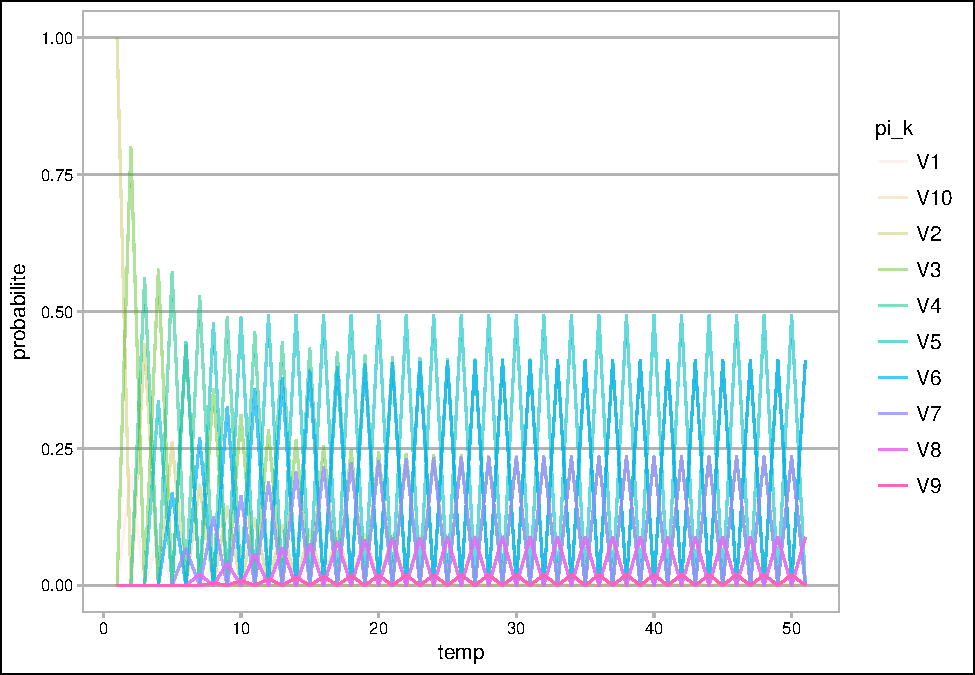
\includegraphics{money_exchange_files/figure-latex/unnamed-chunk-6-1.pdf}

\begin{itemize}
\tightlist
\item
  Nous pouvons observer que X(t) ne converge pas spécialement . Mais que
  toutefois on observe des sauts particuliément autour de
  \(\frac{N}{2}\) . Ce qui correspond à l'obtention d'un régime
  stationnaire au bout d'un certain temps.
\end{itemize}

\section{Processus aléatoire à temps
discret}\label{processus-aleatoire-a-temps-discret}

Nous considérons le premier modéle étudié.\\
soit:
\[ \pi_k \approx \frac{\binom{N_A}{k}\binom{N_B}{N_A-k}}{\binom{N_A+N_B}{N_A}} \]\\
et \[X(t) \rightarrow \pi \] nous posons
\(\Lambda(t) =\frac{X(t)}{N_A}\) et
\(\lambda(t)=\mathbb{E}(\Lambda(t))\)\\
\[\mathbb{E}[X(t+1)]=\sum_{k=0}^{N_A}kP(X(t+1)=k)\]\\
\[P(X(t+1)=k)=\sum_{i \in [k-1,k+1]} P(X(t+1)=k|X(t)=i)P(X(t)=i) \]\\
\[\mathbb{E}(X(t+1))=\sum_0^{N_A}k\sum_{i \in [k-1,k+1]} P(X(t+1)=k|X(t)=i)P(X(t)=i)\]\\
\[= \sum_0^{N_A}k P_{k,k}P_k+\sum_0^{N_A}kP_{k-1,k}P_{k-1} + \sum_{0}^{N_A}kP_{k+1,k}P_{k+1}\]\\
\[= \sum_0^{N_A}k P_{k,k}P_k+\sum_1^{N_A}kP_{k-1,k}P_{k-1}+\sum_{0}^{N_A-1}kP_{k+1,k}P_{k+1}\]\\
\[=\sum_0^{N_A}k P_{k,k}P_k+\sum_0^{N_A}(k+1)P_{k,k+1}P_{k}+\sum_{0}^{N_A}(k-1)P_{k,k}P_{k}\]\\
\[=\sum_0^{N_A}P_k(kP_{k,k} +(k+1)P_{k,k+1}+ (k-1)P_{k,k-1})\]\\
\[=\sum_0^{N_A}P_k (k(P_{k,k}+P_{k,k+1}+P_{k,k-1}) +P_{k,k+1}-P_{k,k-1})\]\\
\[=\sum_0^{N_A}P_k(k+ P_{k,k+1}-P_{k,k-1})\]\\
\[=\sum_0^{N_A}P_k(k+\rho -\frac{k}{N_A}-\frac{k}{N_B})\]\\
\[= \sum_0^{N_A}kP_k -\frac{1+\rho}{N_A}\sum_0^{N_A}kP_k +\rho\sum_0^{N_A}P_k\]\\
\[=\mathbb{E}[X(t)]-\frac{1+\rho}{N_A}\mathbb{E}[X(t)]+ \rho \]\\
\[\mathbb{E}[X(t+1)]=\mathbb{E}[X(t)](1-\frac{1+\rho}{N_A}) +\rho\]\\
\[\Longleftrightarrow  \mathbb{E}[\frac{X(t+1)}{N_A}]=\mathbb{E}[\frac{X(t)}{N_A}](1- \frac{1+\rho}{N_A} ) +\frac{\rho}{N_A} \]\\
\[\Longleftrightarrow \lambda(t+1)=\lambda(t)(1-\frac{1+\rho}{N_A}) +\frac{\rho}{N_A} \]
or
\(\lambda(t)=\mathbb{E}(\Lambda(t))=\frac{1}{N_A}\mathbb{E}(X(t))=\frac{N_A}{N_A+N_B}\)
Avec \(\lambda(t)\) vérifiant la relation de récurrence suivante:\\
\[\lambda(t+1)=\lambda(t)(1-\frac{1+\rho}{N_A})+\frac{\rho}{N_A}\]

• Simulation de \(\lambda\) , pour \(N_A=N_B\) (c'est à dire \(\rho=1\))
avec \(X(0)=99\) et \(X(0)=0\)

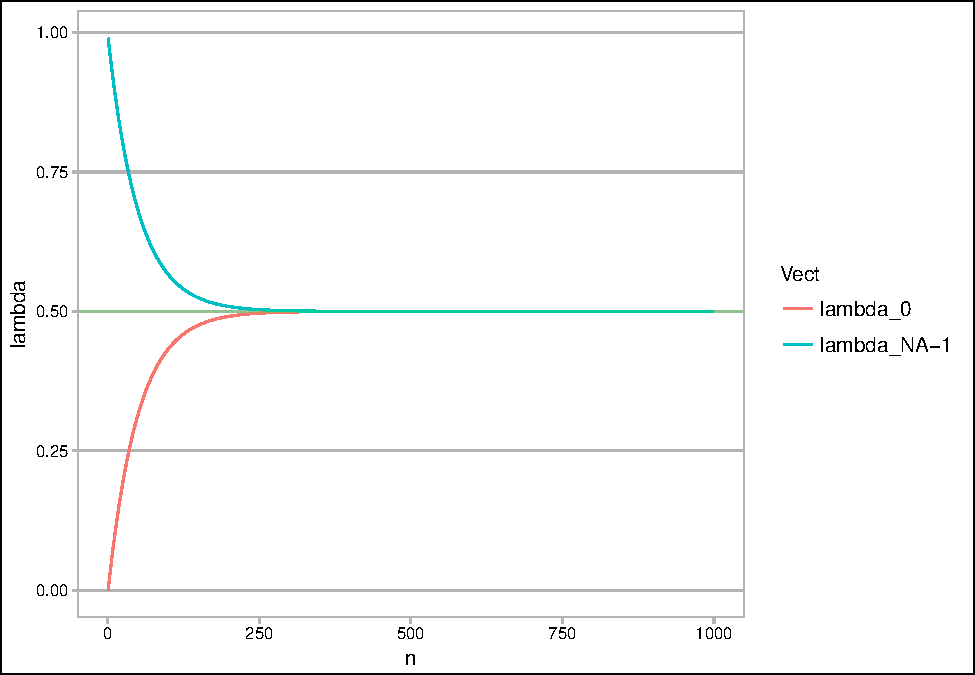
\includegraphics{money_exchange_files/figure-latex/unnamed-chunk-7-1.pdf}

\begin{itemize}
\tightlist
\item
  Nous pouvons observer que lambda, l'espérance de la proportion des
  piéces de \(A\) dans \(A\) convergent vers \(\frac{N_A}{N_A+N_B}=0.5\)
  (à partir de \emph{t} environ à 250 )
\end{itemize}

\newpage  

• Simulation de \(\lambda\) , pour \(N_A \leq N_B\) ( c'est à dire
\(\rho \approx 0\)) avec \(X(0)=N_A-1\) et \(X(0)=0\)

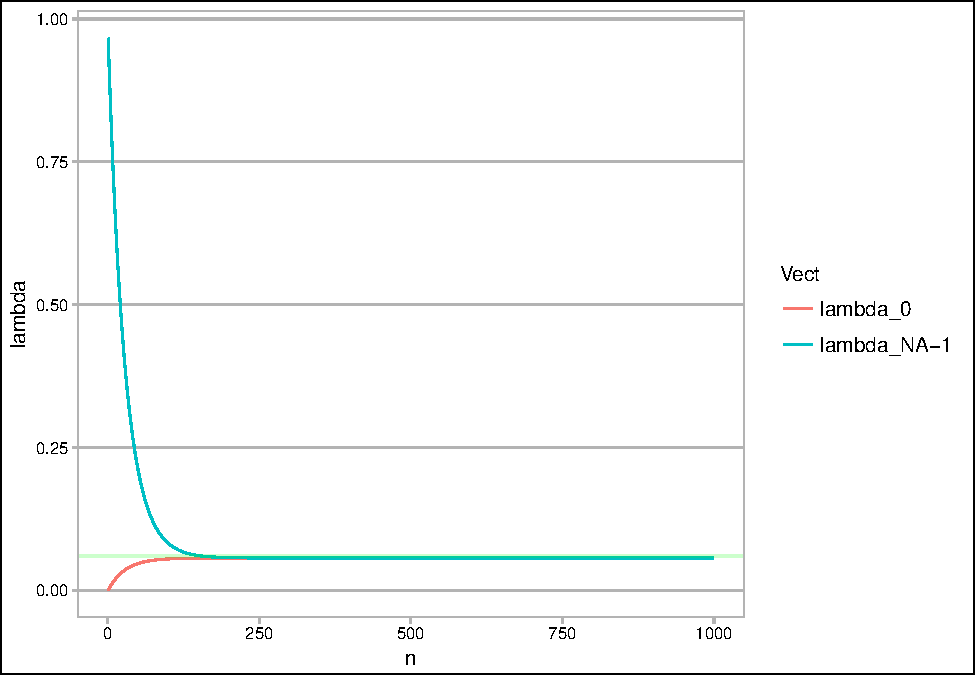
\includegraphics{money_exchange_files/figure-latex/unnamed-chunk-8-1.pdf}

\begin{itemize}
\tightlist
\item
  Nous pouvons voir comme précedemment, une convergence de \(\lambda\)
  vers \(\frac{N_A}{N_A+N_B}\). Nous pouvons souligner le fait que la
  convergence est plus rapide quand \(\rho\) est proche \(0\)
\end{itemize}

En utilisant le relation de récurrence de \(\lambda(t+1)\) dans le cas
\(N_A=N_B\) nous obtenons :\\
\[\Lambda(t+1)=\frac{1}{N} + (1-\frac{2}{N})\Lambda(t)+\frac{\sqrt[]{2\Lambda(t)(1-\Lambda(t))}}{N}\epsilon_{t+1}\]
Avec \(\epsilon_t+1 \sim \mathcal{N}(0,1)\) le bruit au temps \(t+1\)\\
Sachant que \(\lambda(t+1) \Rightarrow \frac{1}{2}\) , pour centrer
\(\Lambda(t+1)\) On pose : \[H(t)=\Lambda(t)-\frac{1}{2}
\Longleftrightarrow H(t+1)=\Lambda(t+1)-\frac{1}{2}\]
\[=\frac{1}{N} +(1-\frac{2}{N})H(t) +\frac{1}{2} -\frac{1}{N} +\frac{\sqrt[]{(2(H(t)+\frac{1}{2})(\frac{1}{2}-H(t))} }{N}\epsilon_{t+1}\]
\[=\frac{1}{2}+ (1-\frac{2}{N})H(t)   +\frac{\sqrt[]{(2(-H(t)^2)+\frac{1}{4}) }}{N}\epsilon_{t+1}\]
\[=\frac{1}{2}+ (1-\frac{2}{N})H(t)   +\frac{\sqrt[]{(2(-H(t)^2)+\frac{1}{4}) }}{N}\epsilon_{t+1}\]

Sachant quand que \(H(t)\) proche de \(0\) :

\[\Longleftrightarrow \Lambda(t+1) \approx \frac{1}{2}+(1-\frac{2}{N})H(t)+\frac{1}{\sqrt{2}N}\epsilon_{t+1}\]
\[ \Longleftrightarrow H(t+1) \approx (1-\frac{2}{N})H(t) +\frac{1}{\sqrt{2}N}\epsilon_{t+1}  \]

En supposant que les \(\epsilon_i\) soit iid ,

\[Y(t+1)=aY(t)+\sigma \epsilon_{t+1}\]\\
Dans ce cas nous obtiendrons un régime stationnaire (comme dans le
\textbf{Cas Particulier} ).\\
Et dans ce cas pour tout
\(t \in \mathbb{N}, H(t) \rightarrow \mathcal{N}(0,\frac{1}{8N}))\).

• Simulation de \(H(t)\) en fonction de \(N\)

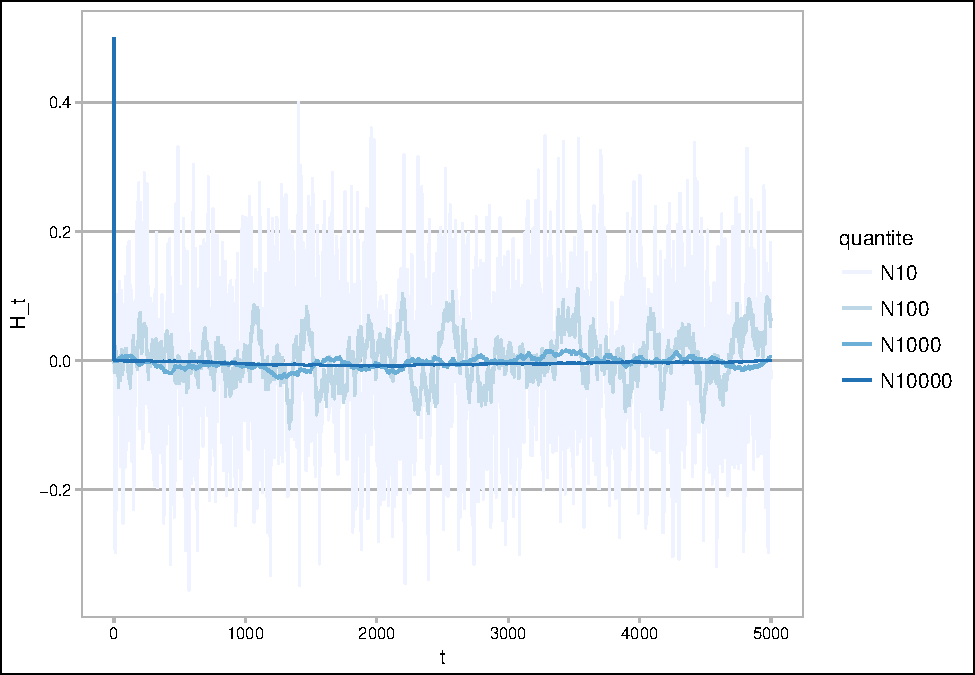
\includegraphics{money_exchange_files/figure-latex/unnamed-chunk-9-1.pdf}

\begin{itemize}
\tightlist
\item
  Avec ce graphique nous pouvons voir que l'on obtient un regime
  stationnaire (c'est dire un sentier stable dans le processus) , avec
  un écart-type \(\sigma\) qui décroit fortement avec \(N\) (qui
  augmente ). Nous pouvons néanmoins noté que la stabilité dans le
  processus est plus garantit (dans le long terme ) par \(N\) assez
  grand.
\end{itemize}

\section{Conclusion}\label{conclusion}

Pour conclure nous pouvons dire qu'à travers les modéles présentés,
l'équilibre recherché n'est pas forcément atteint. Toutefois modéles
guarantit un régime stationnaire autour du point de convergence. Ce
régime stationnaire serait dû à un déséquilibre causé par les bruits
corrélés ( à chaque \(t\)). Nous avons pû constater néanmoins que une
différence grande en quantité de monnaie fabriquée par deux pays,
converge non seulement plutôt vers la mesure invariante. Mais aussi
donne régime stationnaire dans lequel la dispersion est beaucoup moins
forte. Nous pouvons souligner cette faible dispersion dans le cas ou la
masse monétaire dans les deux pays est trés grande. Toutefois ce modéle
ne prend pas en compte ni le type de masse monétaire ni les differences
que peuvent avoir deux pays. Il ne prend aussi pas en compte le décalage
inter-temporels dans les échanges qui fait que la masse monétaire
globale varie aussi dans le temps.

\section{Code}\label{code}

\begin{Shaded}
\begin{Highlighting}[]
\KeywordTok{library}\NormalTok{(ggplot2)}
\KeywordTok{library}\NormalTok{(magrittr)}
\KeywordTok{library}\NormalTok{(rmarkdown)}
\KeywordTok{library}\NormalTok{(dplyr)}
\KeywordTok{library}\NormalTok{(tidyr)}
\KeywordTok{library}\NormalTok{(RColorBrewer)}
\KeywordTok{library}\NormalTok{(reshape2)}
\KeywordTok{library}\NormalTok{(ggthemes)}
\KeywordTok{library}\NormalTok{(MASS)}
\KeywordTok{library}\NormalTok{(viridis)}
\KeywordTok{library}\NormalTok{(GSIF)}
\KeywordTok{library}\NormalTok{(ggtern)}
\KeywordTok{library}\NormalTok{(geomnet)}
\KeywordTok{library}\NormalTok{(ggmap)}
\KeywordTok{library}\NormalTok{(ggfortify)}
\KeywordTok{library}\NormalTok{(vars)}
\KeywordTok{library}\NormalTok{(maps)}
\KeywordTok{library}\NormalTok{(rgdal)}
\KeywordTok{library}\NormalTok{(animation)}
\KeywordTok{library}\NormalTok{(class)}
\KeywordTok{library}\NormalTok{(combinat)}
\KeywordTok{library}\NormalTok{(grDevices)}
\KeywordTok{library}\NormalTok{(markovchain)}
\KeywordTok{library}\NormalTok{(igraph)}
\KeywordTok{library}\NormalTok{(diagram)}
\KeywordTok{library}\NormalTok{(stringr)  }

\CommentTok{#fonction mmatrice de transition}
\NormalTok{makemat=}\ControlFlowTok{function}\NormalTok{(N_A,N_B)\{}
\NormalTok{  ro=N_A}\OperatorTok{/}\NormalTok{N_B}
\NormalTok{  matrice=}\KeywordTok{matrix}\NormalTok{(}\DecValTok{0}\NormalTok{,}\DataTypeTok{nrow=}\NormalTok{N_A,}\DataTypeTok{ncol=}\NormalTok{N_A) }
\NormalTok{  matrice[}\DecValTok{1}\NormalTok{,}\DecValTok{2}\NormalTok{]=ro}
\NormalTok{  matrice[}\DecValTok{1}\NormalTok{,}\DecValTok{1}\NormalTok{]=}\DecValTok{1}\OperatorTok{-}\NormalTok{ro}
\NormalTok{  matrice[N_A,N_A}\OperatorTok{-}\DecValTok{1}\NormalTok{]=}\DecValTok{1}
  \ControlFlowTok{for}\NormalTok{(i }\ControlFlowTok{in} \DecValTok{1}\OperatorTok{:}\NormalTok{N_A}\OperatorTok{-}\DecValTok{1}\NormalTok{)\{}
    \ControlFlowTok{for}\NormalTok{(j }\ControlFlowTok{in} \DecValTok{1}\OperatorTok{:}\NormalTok{N_A}\OperatorTok{-}\DecValTok{1}\NormalTok{)\{}
      \ControlFlowTok{if}\NormalTok{(i}\OperatorTok{==}\NormalTok{j }\OperatorTok{&}\NormalTok{i}\OperatorTok{!=}\DecValTok{1}\NormalTok{)\{}
\NormalTok{        matrice[i,j]=(}\DecValTok{1}\OperatorTok{-}\NormalTok{i}\OperatorTok{/}\NormalTok{N_A)}\OperatorTok{*}\NormalTok{(}\DecValTok{1}\OperatorTok{-}\NormalTok{ro}\OperatorTok{+}\DecValTok{2}\OperatorTok{*}\NormalTok{ro}\OperatorTok{*}\NormalTok{(i}\OperatorTok{/}\NormalTok{N_A))}
\NormalTok{       matrice[i,j}\OperatorTok{-}\DecValTok{1}\NormalTok{]=(i}\OperatorTok{/}\NormalTok{N_A)}\OperatorTok{*}\NormalTok{(}\DecValTok{1}\OperatorTok{-}\NormalTok{ro}\OperatorTok{+}\NormalTok{ro}\OperatorTok{*}\NormalTok{(i}\OperatorTok{/}\NormalTok{N_A))}
\NormalTok{       matrice[i,j}\OperatorTok{+}\DecValTok{1}\NormalTok{]=ro}\OperatorTok{*}\NormalTok{(}\DecValTok{1}\OperatorTok{-}\NormalTok{i}\OperatorTok{/}\NormalTok{N_A)}\OperatorTok{^}\DecValTok{2}
\NormalTok{      \}}
      
        
      
\NormalTok{    \}}
\NormalTok{  \}}
\KeywordTok{return}\NormalTok{(matrice)  }
\NormalTok{\}}


\NormalTok{matrice=}\KeywordTok{makemat}\NormalTok{(}\DecValTok{10}\NormalTok{,}\DecValTok{10}\NormalTok{)}


\NormalTok{pi0=}\KeywordTok{c}\NormalTok{(}\DecValTok{0}\NormalTok{,}\DecValTok{1}\NormalTok{,}\DecValTok{0}\NormalTok{,}\DecValTok{0}\NormalTok{,}\DecValTok{0}\NormalTok{,}\DecValTok{0}\NormalTok{,}\DecValTok{0}\NormalTok{,}\DecValTok{0}\NormalTok{,}\DecValTok{0}\NormalTok{,}\DecValTok{0}\NormalTok{)}
  


\CommentTok{#mesure invariant}
\NormalTok{mesureinv=}\ControlFlowTok{function}\NormalTok{(N_A,N_B)\{}
\NormalTok{  pi=}\KeywordTok{vector}\NormalTok{(}\StringTok{"double"}\NormalTok{,}\DataTypeTok{length=}\NormalTok{N_A)}
  \ControlFlowTok{for}\NormalTok{(i }\ControlFlowTok{in} \DecValTok{1}\OperatorTok{:}\NormalTok{N_A)\{}
\NormalTok{    pi[i]=(}\KeywordTok{choose}\NormalTok{(N_A,i)}\OperatorTok{*}\KeywordTok{choose}\NormalTok{(N_B,N_A}\OperatorTok{-}\NormalTok{i))}\OperatorTok{/}\KeywordTok{choose}\NormalTok{(N_A}\OperatorTok{+}\NormalTok{N_B,N_A)}
\NormalTok{  \}}
\NormalTok{  pi}
\NormalTok{\}}

\NormalTok{inv10=}\KeywordTok{mesureinv}\NormalTok{(}\DecValTok{10}\NormalTok{,}\DecValTok{14}\NormalTok{)}

\CommentTok{# fonction qui retourne un vecteur de  mesure à  chaque temps t }
\NormalTok{temp=}\ControlFlowTok{function}\NormalTok{(N_A,N_B,initial,imax,iteration)\{}
\NormalTok{  t=}\DecValTok{0}
\NormalTok{  mat=}\KeywordTok{makemat}\NormalTok{(N_A,N_B)}
\NormalTok{  mesure=}\KeywordTok{mesureinv}\NormalTok{(N_A,N_B )}
\NormalTok{  pi0=}\KeywordTok{vector}\NormalTok{(}\StringTok{"double"}\NormalTok{,}\DataTypeTok{length=}\NormalTok{N_A)}
\NormalTok{  pi0[initial]=}\DecValTok{1}
\NormalTok{  pi=pi0}\OperatorTok\NormalTok{mat}
\NormalTok{  historique=pi}
  \CommentTok{# tant que pi different de mesure invariante, faire instructions}
  \ControlFlowTok{while}\NormalTok{(}\KeywordTok{round}\NormalTok{(pi,iteration)}\OperatorTok{!=}\KeywordTok{round}\NormalTok{(mesure,iteration) }\OperatorTok{&&}\StringTok{ }\NormalTok{t}\OperatorTok{<}\NormalTok{imax )\{}
\NormalTok{    pi=pi}\OperatorTok\NormalTok{mat}
    
\NormalTok{    historique=}\KeywordTok{rbind}\NormalTok{(historique,pi)}
\NormalTok{    t=t}\OperatorTok{+}\DecValTok{1}
\NormalTok{  \}}
\KeywordTok{list}\NormalTok{(}\DataTypeTok{temps=}\NormalTok{pi,}\DataTypeTok{histo=}\NormalTok{historique,}\DataTypeTok{t=}\NormalTok{t)}
\NormalTok{\}}

\NormalTok{mesure=}\KeywordTok{temp}\NormalTok{(}\DecValTok{10}\NormalTok{,}\DecValTok{14}\NormalTok{,}\DecValTok{10}\NormalTok{,}\DecValTok{200}\NormalTok{)}
\NormalTok{historique=}\KeywordTok{as.data.frame}\NormalTok{(mesure}\OperatorTok{$}\NormalTok{histo)}
\NormalTok{historique}
\KeywordTok{round}\NormalTok{(inv10,}\DecValTok{7}\NormalTok{)}
\KeywordTok{round}\NormalTok{(mesure}\OperatorTok{$}\NormalTok{temps,}\DecValTok{3}\NormalTok{)}
\NormalTok{mesure}\OperatorTok{$}\NormalTok{t}
\NormalTok{historique =}\StringTok{ }\NormalTok{historique }\OperatorTok
\StringTok{                 }\KeywordTok{gather}\NormalTok{(}\DataTypeTok{key =}\NormalTok{ Etats,}\DataTypeTok{value=}\NormalTok{mesure)}
                 
\NormalTok{historique}\OperatorTok{$}\NormalTok{Etats=}\KeywordTok{as.factor}\NormalTok{(historique}\OperatorTok{$}\NormalTok{Etats)}
               
\NormalTok{historique=historique }\OperatorTok
\StringTok{           }\KeywordTok{group_by}\NormalTok{(Etats)}\OperatorTok
\StringTok{                 }\KeywordTok{mutate}\NormalTok{(}\DataTypeTok{n=}\DecValTok{1}\OperatorTok{:}\KeywordTok{n}\NormalTok{())}

\CommentTok{# Graphique convergence pi}
\KeywordTok{ggplot}\NormalTok{(historique,}\KeywordTok{aes}\NormalTok{(}\DataTypeTok{x=}\NormalTok{n,}\DataTypeTok{y=}\NormalTok{mesure,}\DataTypeTok{col=}\NormalTok{Etats,}\DataTypeTok{main=}\StringTok{"Convergence Etats"}\NormalTok{))}\OperatorTok{+}
\StringTok{   }\KeywordTok{geom_line}\NormalTok{()}\OperatorTok{+}
\StringTok{ }\KeywordTok{xlab}\NormalTok{(}\StringTok{"temp"}\NormalTok{)}\OperatorTok{+}
\StringTok{  }\KeywordTok{theme_calc}\NormalTok{()}
\NormalTok{mesure=}\KeywordTok{temp}\NormalTok{(}\DecValTok{20}\NormalTok{,}\DecValTok{20}\NormalTok{,}\DecValTok{20}\NormalTok{,}\DecValTok{100}\NormalTok{,}\DecValTok{10}\NormalTok{)}
\NormalTok{historique=}\KeywordTok{as.data.frame}\NormalTok{(mesure}\OperatorTok{$}\NormalTok{histo)}

\NormalTok{historique =}\StringTok{ }\NormalTok{historique }\OperatorTok
\StringTok{                 }\KeywordTok{gather}\NormalTok{(}\DataTypeTok{key =}\NormalTok{ pi_k,}\DataTypeTok{value=}\NormalTok{probabilite)}
                 
\NormalTok{historique}\OperatorTok{$}\NormalTok{pi_k=}\KeywordTok{as.factor}\NormalTok{(historique}\OperatorTok{$}\NormalTok{pi_k)}
               
\NormalTok{historique=historique }\OperatorTok
\StringTok{           }\KeywordTok{group_by}\NormalTok{(pi_k)}\OperatorTok
\StringTok{                 }\KeywordTok{mutate}\NormalTok{(}\DataTypeTok{n=}\DecValTok{1}\OperatorTok{:}\KeywordTok{n}\NormalTok{())}

\CommentTok{# Graphique convergence pi}
\KeywordTok{ggplot}\NormalTok{(historique,}\KeywordTok{aes}\NormalTok{(}\DataTypeTok{x=}\NormalTok{n,}\DataTypeTok{y=}\NormalTok{probabilite,}\DataTypeTok{col=}\NormalTok{pi_k,}\DataTypeTok{fill=}\NormalTok{pi_k,}\DataTypeTok{main=}\StringTok{"Convergence Etats"}\NormalTok{))}\OperatorTok{+}
\StringTok{   }\KeywordTok{geom_line}\NormalTok{()}\OperatorTok{+}
\StringTok{ }\KeywordTok{xlab}\NormalTok{(}\StringTok{"temp"}\NormalTok{)}\OperatorTok{+}
\StringTok{  }\KeywordTok{theme_calc}\NormalTok{()}

\CommentTok{# fonction pour matrice de transition (cas particulier)}
\NormalTok{makemat2=}\ControlFlowTok{function}\NormalTok{(N_A)\{}
\NormalTok{  matrice=}\KeywordTok{matrix}\NormalTok{(}\DecValTok{0}\NormalTok{,}\DataTypeTok{nrow=}\NormalTok{N_A,}\DataTypeTok{ncol=}\NormalTok{N_A) }
\NormalTok{  matrice[}\DecValTok{1}\NormalTok{,}\DecValTok{2}\NormalTok{]=}\DecValTok{1}
\NormalTok{  matrice[N_A,N_A}\OperatorTok{-}\DecValTok{1}\NormalTok{]=}\DecValTok{1}
  \ControlFlowTok{for}\NormalTok{(i }\ControlFlowTok{in} \DecValTok{1}\OperatorTok{:}\NormalTok{N_A}\OperatorTok{-}\DecValTok{1}\NormalTok{)\{}
    \ControlFlowTok{for}\NormalTok{(j }\ControlFlowTok{in} \DecValTok{1}\OperatorTok{:}\NormalTok{N_A}\OperatorTok{-}\DecValTok{1}\NormalTok{)\{}
      \ControlFlowTok{if}\NormalTok{(i}\OperatorTok{==}\NormalTok{j }\OperatorTok{&}\NormalTok{i}\OperatorTok{!=}\DecValTok{1}\NormalTok{)\{}
\NormalTok{       matrice[i,j}\OperatorTok{-}\DecValTok{1}\NormalTok{]=i}\OperatorTok{/}\NormalTok{N_A}
\NormalTok{       matrice[i,j}\OperatorTok{+}\DecValTok{1}\NormalTok{]=(}\DecValTok{1}\OperatorTok{-}\NormalTok{i}\OperatorTok{/}\NormalTok{N_A)}
\NormalTok{      \}}
      
        
      
\NormalTok{    \}}
\NormalTok{  \}}
\KeywordTok{return}\NormalTok{(matrice)  }
\NormalTok{\}}


\NormalTok{matrice1=}\KeywordTok{makemat2}\NormalTok{(}\DecValTok{20}\NormalTok{)}


\CommentTok{#mesure invariant 2 (cas partiulier)}
\NormalTok{mesureinv2=}\ControlFlowTok{function}\NormalTok{(N_A)\{}
\NormalTok{  pi=}\KeywordTok{vector}\NormalTok{(}\StringTok{"double"}\NormalTok{,}\DataTypeTok{length=}\NormalTok{N_A)}
  \ControlFlowTok{for}\NormalTok{(i }\ControlFlowTok{in} \DecValTok{1}\OperatorTok{:}\NormalTok{N_A)\{}
\NormalTok{    pi[i]=(}\KeywordTok{choose}\NormalTok{(N_A,i)}\OperatorTok{*}\NormalTok{(}\DecValTok{1}\OperatorTok{/}\DecValTok{2}\NormalTok{)}\OperatorTok{^}\NormalTok{N_A)}
\NormalTok{  \}}
\NormalTok{  pi}
\NormalTok{\}}
\NormalTok{mesure1=}\KeywordTok{mesureinv2}\NormalTok{(}\DecValTok{10}\NormalTok{)}

\NormalTok{temp1=}\ControlFlowTok{function}\NormalTok{(N_A,initial,imax,arrondi)\{}
\NormalTok{  t=}\DecValTok{0}
\NormalTok{  mat=}\KeywordTok{makemat2}\NormalTok{(N_A)}
\NormalTok{  mesure=}\KeywordTok{mesureinv2}\NormalTok{(N_A )}
\NormalTok{  pi0=}\KeywordTok{vector}\NormalTok{(}\StringTok{"double"}\NormalTok{,}\DataTypeTok{length=}\NormalTok{N_A)}
\NormalTok{  pi0[initial]=}\DecValTok{1}
\NormalTok{  pi=pi0}\OperatorTok\NormalTok{mat}
\NormalTok{  historique=pi}
  \CommentTok{# tant que pi different de mesure invariante, faire instructions}
  \ControlFlowTok{while}\NormalTok{(}\KeywordTok{round}\NormalTok{(pi,arrondi)}\OperatorTok{!=}\KeywordTok{round}\NormalTok{(mesure,arrondi) }\OperatorTok{&&}\StringTok{ }\NormalTok{t}\OperatorTok{<}\NormalTok{imax )\{}
\NormalTok{    pi=pi}\OperatorTok\NormalTok{mat}
    
\NormalTok{    historique=}\KeywordTok{rbind}\NormalTok{(historique,pi)}
\NormalTok{    t=t}\OperatorTok{+}\DecValTok{1}
\NormalTok{  \}}
\KeywordTok{list}\NormalTok{(}\DataTypeTok{temps=}\NormalTok{pi,}\DataTypeTok{histo=}\NormalTok{historique,}\DataTypeTok{t=}\NormalTok{t)}
\NormalTok{\}}

\NormalTok{mesure1=}\KeywordTok{temp1}\NormalTok{(}\DecValTok{10}\NormalTok{,}\DecValTok{1}\NormalTok{,}\DecValTok{50}\NormalTok{,}\DecValTok{50}\NormalTok{)}

\NormalTok{historique1=}\KeywordTok{as.data.frame}\NormalTok{(mesure1}\OperatorTok{$}\NormalTok{histo)}


\NormalTok{historique1 =}\StringTok{ }\NormalTok{historique1 }\OperatorTok
\StringTok{                 }\KeywordTok{gather}\NormalTok{(}\DataTypeTok{key =}\NormalTok{ pi_k,}\DataTypeTok{value=}\NormalTok{probabilite)}
                 
\NormalTok{historique1}\OperatorTok{$}\NormalTok{pi_k=}\KeywordTok{as.factor}\NormalTok{(historique1}\OperatorTok{$}\NormalTok{pi_k)}
               
\NormalTok{historique1=historique1 }\OperatorTok
\StringTok{           }\KeywordTok{group_by}\NormalTok{(pi_k)}\OperatorTok
\StringTok{                 }\KeywordTok{mutate}\NormalTok{(}\DataTypeTok{n=}\DecValTok{1}\OperatorTok{:}\KeywordTok{n}\NormalTok{())}

\KeywordTok{ggplot}\NormalTok{(historique1,}\KeywordTok{aes}\NormalTok{(}\DataTypeTok{x=}\NormalTok{n,}\DataTypeTok{y=}\NormalTok{probabilite,}\DataTypeTok{col=}\NormalTok{pi_k,}\DataTypeTok{main=}\StringTok{"Convergence Etats"}\NormalTok{,}\DataTypeTok{alpha=}\NormalTok{pi_k))}\OperatorTok{+}
\StringTok{   }\KeywordTok{geom_line}\NormalTok{()}\OperatorTok{+}
\StringTok{ }\KeywordTok{xlab}\NormalTok{(}\StringTok{"temp"}\NormalTok{)}\OperatorTok{+}
\StringTok{  }\KeywordTok{theme}\NormalTok{(}\DataTypeTok{legend.position=}\StringTok{"none"}\NormalTok{)}\OperatorTok{+}
\StringTok{  }\KeywordTok{theme_calc}\NormalTok{()}\OperatorTok{+}
\StringTok{ }\KeywordTok{scale_color_discrete}\NormalTok{()  }
  
\CommentTok{#simulation Lambda}

\NormalTok{simul=}\ControlFlowTok{function}\NormalTok{(N_A,N_B,t,lambda0)\{}
\NormalTok{  lambda=lambda0}\OperatorTok{/}\NormalTok{N_A}
\NormalTok{  rho=N_A}\OperatorTok{/}\NormalTok{N_B}
\NormalTok{  vect=}\KeywordTok{vector}\NormalTok{(}\StringTok{"double"}\NormalTok{,}\DataTypeTok{length=}\NormalTok{t)}
\NormalTok{  vect[}\DecValTok{1}\NormalTok{]=lambda}
  \ControlFlowTok{for}\NormalTok{(i }\ControlFlowTok{in} \DecValTok{2}\OperatorTok{:}\NormalTok{t)\{}
\NormalTok{    vect[i]=lambda}\OperatorTok{*}\NormalTok{(}\DecValTok{1}\OperatorTok{-}\NormalTok{(}\DecValTok{1}\OperatorTok{+}\NormalTok{rho)}\OperatorTok{/}\NormalTok{N_A)}\OperatorTok{+}\NormalTok{rho}\OperatorTok{/}\NormalTok{N_A}
\NormalTok{    lambda=vect[i]  }
\NormalTok{  \}}
\NormalTok{  vect=}\KeywordTok{cbind}\NormalTok{(vect,}\DataTypeTok{n=}\DecValTok{1}\OperatorTok{:}\KeywordTok{length}\NormalTok{(vect))}
\NormalTok{\}}

\CommentTok{# Simulation de lambda 1}

\NormalTok{f=}\KeywordTok{simul}\NormalTok{(}\DecValTok{100}\NormalTok{,}\DecValTok{100}\NormalTok{,}\DecValTok{1000}\NormalTok{,}\DecValTok{99}\NormalTok{)}
\NormalTok{f1=}\KeywordTok{simul}\NormalTok{(}\DecValTok{100}\NormalTok{,}\DecValTok{100}\NormalTok{,}\DecValTok{1000}\NormalTok{,}\DecValTok{0}\NormalTok{)}
\NormalTok{fam=}\KeywordTok{as.data.frame}\NormalTok{(f)}
\KeywordTok{names}\NormalTok{(fam)=}\KeywordTok{c}\NormalTok{(}\StringTok{"lambda_NA-1"}\NormalTok{,}\StringTok{"n"}\NormalTok{)}
\NormalTok{fam1=}\KeywordTok{as.data.frame}\NormalTok{(f1)  }
\NormalTok{fam=fam }\OperatorTok
\StringTok{     }\KeywordTok{mutate}\NormalTok{(}\DataTypeTok{lambda_0=}\NormalTok{fam1}\OperatorTok{$}\NormalTok{vect)}\OperatorTok
\StringTok{     }\KeywordTok{gather}\NormalTok{(}\DataTypeTok{key=}\NormalTok{Vect,}\DataTypeTok{value =}\NormalTok{valeur,}\OperatorTok{-}\NormalTok{n )}\OperatorTok
\StringTok{  }\KeywordTok{tbl_df}\NormalTok{()}

\NormalTok{fam}\OperatorTok{$}\NormalTok{Vect=}\KeywordTok{as.factor}\NormalTok{(fam}\OperatorTok{$}\NormalTok{Vect)}

\KeywordTok{ggplot}\NormalTok{(fam,}\KeywordTok{aes}\NormalTok{(}\DataTypeTok{x=}\NormalTok{n,}\DataTypeTok{y=}\NormalTok{valeur,}\DataTypeTok{col=}\NormalTok{Vect))}\OperatorTok{+}
\StringTok{  }\KeywordTok{geom_line}\NormalTok{()}\OperatorTok{+}
\StringTok{  }\KeywordTok{theme_calc}\NormalTok{()}\OperatorTok{+}
\StringTok{  }\KeywordTok{ylab}\NormalTok{(}\StringTok{"lambda"}\NormalTok{)}\OperatorTok{+}
\StringTok{    }\KeywordTok{geom_hline}\NormalTok{(}\DataTypeTok{yintercept =}\DecValTok{1}\OperatorTok{/}\DecValTok{2}\NormalTok{,}\DataTypeTok{alpha=}\FloatTok{0.2}\NormalTok{,}\DataTypeTok{show.legend =}\NormalTok{ T,}\DataTypeTok{col=}\StringTok{"green"}\NormalTok{)}

\CommentTok{# Simulation de lambda 2  }

\NormalTok{f=}\KeywordTok{simul}\NormalTok{(}\DecValTok{30}\NormalTok{,}\DecValTok{500}\NormalTok{,}\DecValTok{1000}\NormalTok{,}\DecValTok{29}\NormalTok{)}
\NormalTok{f1=}\KeywordTok{simul}\NormalTok{(}\DecValTok{30}\NormalTok{,}\DecValTok{500}\NormalTok{,}\DecValTok{1000}\NormalTok{,}\DecValTok{0}\NormalTok{)}

\NormalTok{fam=}\KeywordTok{as.data.frame}\NormalTok{(f)}
\KeywordTok{names}\NormalTok{(fam)=}\KeywordTok{c}\NormalTok{(}\StringTok{"lambda_NA-1"}\NormalTok{,}\StringTok{"n"}\NormalTok{)}
\NormalTok{fam1=}\KeywordTok{as.data.frame}\NormalTok{(f1)  }
\NormalTok{fam=fam }\OperatorTok
\StringTok{     }\KeywordTok{mutate}\NormalTok{(}\DataTypeTok{lambda_0=}\NormalTok{fam1}\OperatorTok{$}\NormalTok{vect)}\OperatorTok
\StringTok{     }\KeywordTok{gather}\NormalTok{(}\DataTypeTok{key=}\NormalTok{Vect,}\DataTypeTok{value =}\NormalTok{valeur,}\OperatorTok{-}\NormalTok{n )}\OperatorTok
\StringTok{  }\KeywordTok{tbl_df}\NormalTok{()}

\NormalTok{fam}\OperatorTok{$}\NormalTok{Vect=}\KeywordTok{as.factor}\NormalTok{(fam}\OperatorTok{$}\NormalTok{Vect)}

\KeywordTok{ggplot}\NormalTok{(fam,}\KeywordTok{aes}\NormalTok{(}\DataTypeTok{x=}\NormalTok{n,}\DataTypeTok{y=}\NormalTok{valeur,}\DataTypeTok{col=}\NormalTok{Vect))}\OperatorTok{+}
\StringTok{  }\KeywordTok{geom_line}\NormalTok{()}\OperatorTok{+}
\StringTok{  }\KeywordTok{theme_calc}\NormalTok{()}\OperatorTok{+}
\StringTok{  }\KeywordTok{ylab}\NormalTok{(}\StringTok{"lambda"}\NormalTok{)}\OperatorTok{+}
\StringTok{    }\KeywordTok{geom_hline}\NormalTok{(}\DataTypeTok{yintercept =}\DecValTok{30}\OperatorTok{/}\DecValTok{500}\NormalTok{,}\DataTypeTok{alpha=}\FloatTok{0.2}\NormalTok{,}\DataTypeTok{show.legend =}\NormalTok{ T,}\DataTypeTok{col=}\StringTok{"green"}\NormalTok{)}

 \CommentTok{# Simulation H_t  }
\CommentTok{# fonction qui renvoie un tableau avec t et H(t)}
\NormalTok{simul2=}\ControlFlowTok{function}\NormalTok{(N,t)\{}
\NormalTok{  X_}\DecValTok{0}\NormalTok{=N}\OperatorTok{-}\DecValTok{1}
\NormalTok{lambda_}\DecValTok{0}\NormalTok{=X_}\DecValTok{0}\OperatorTok{/}\NormalTok{N}\OperatorTok{-}\DecValTok{1}\OperatorTok{/}\DecValTok{2}
\NormalTok{vect=}\KeywordTok{vector}\NormalTok{(}\StringTok{"double"}\NormalTok{,}\DataTypeTok{length=}\NormalTok{t}\OperatorTok{+}\DecValTok{1}\NormalTok{)}
\NormalTok{lambda_t=lambda_}\DecValTok{0}
\NormalTok{vect[}\DecValTok{1}\NormalTok{]=lambda_t  }
\NormalTok{H_t=lambda_t}\OperatorTok{-}\DecValTok{1}\OperatorTok{/}\DecValTok{2}
\ControlFlowTok{for}\NormalTok{(i }\ControlFlowTok{in} \DecValTok{2}\OperatorTok{:}\NormalTok{t}\OperatorTok{+}\DecValTok{1}\NormalTok{)\{}

\NormalTok{  vect[i]=(}\DecValTok{1}\OperatorTok{-}\DecValTok{2}\OperatorTok{/}\NormalTok{N)}\OperatorTok{*}\NormalTok{H_t }\OperatorTok{+}\StringTok{ }\DecValTok{1}\OperatorTok{/}\NormalTok{(N}\OperatorTok{*}\KeywordTok{sqrt}\NormalTok{(}\DecValTok{2}\NormalTok{))}\OperatorTok{*}\KeywordTok{rnorm}\NormalTok{(}\DecValTok{1}\NormalTok{,}\DataTypeTok{mean=}\DecValTok{0}\NormalTok{,}\DataTypeTok{sd=}\DecValTok{1}\NormalTok{)}
\NormalTok{  H_t=vect[i]}
\NormalTok{\} }
\NormalTok{ vect =}\KeywordTok{tbl_df}\NormalTok{(}\KeywordTok{cbind}\NormalTok{(}\DataTypeTok{H_t=}\NormalTok{vect,}\DataTypeTok{t=}\DecValTok{0}\OperatorTok{:}\NormalTok{t))  }
\NormalTok{\} }
\NormalTok{f1=}\KeywordTok{simul2}\NormalTok{(}\DecValTok{10}\NormalTok{,}\DecValTok{5000}\NormalTok{)}
\NormalTok{f2=}\KeywordTok{simul2}\NormalTok{(}\DecValTok{100}\NormalTok{,}\DecValTok{5000}\NormalTok{)}
\NormalTok{f3=}\KeywordTok{simul2}\NormalTok{(}\DecValTok{1000}\NormalTok{,}\DecValTok{5000}\NormalTok{)}
\NormalTok{f4=}\KeywordTok{simul2}\NormalTok{(}\DecValTok{10000}\NormalTok{,}\DecValTok{5000}\NormalTok{)}


\NormalTok{f=}\KeywordTok{tbl_df}\NormalTok{(}\KeywordTok{cbind}\NormalTok{(}\DataTypeTok{t=}\NormalTok{f1}\OperatorTok{$}\NormalTok{t,}\DataTypeTok{N10=}\NormalTok{f1}\OperatorTok{$}\NormalTok{H_t,}\DataTypeTok{N100=}\NormalTok{f2}\OperatorTok{$}\NormalTok{H_t,}\DataTypeTok{N1000=}\NormalTok{f3}\OperatorTok{$}\NormalTok{H_t,}\DataTypeTok{N10000=}\NormalTok{f4}\OperatorTok{$}\NormalTok{H_t))}\OperatorTok
\StringTok{          }\KeywordTok{gather}\NormalTok{(}\DataTypeTok{key=}\NormalTok{quantite,}\DataTypeTok{value=}\NormalTok{H_t,}\OperatorTok{-}\NormalTok{t)}

\NormalTok{f}\OperatorTok{$}\NormalTok{quantite=}\KeywordTok{as.factor}\NormalTok{(f}\OperatorTok{$}\NormalTok{quantite)}

\KeywordTok{ggplot}\NormalTok{(f,}\KeywordTok{aes}\NormalTok{(}\DataTypeTok{y=}\NormalTok{H_t,}\DataTypeTok{x=}\NormalTok{t,}\DataTypeTok{col=}\NormalTok{quantite))}\OperatorTok{+}
\StringTok{  }\KeywordTok{geom_line}\NormalTok{()}\OperatorTok{+}
\StringTok{  }\KeywordTok{theme_calc}\NormalTok{()}\OperatorTok{+}
\KeywordTok{scale_color_brewer}\NormalTok{()  }
\end{Highlighting}
\end{Shaded}


\end{document}
